%\documentclass[aps,showpacs,prl,twocolumn,superscriptaddress]{revtex4}
\documentclass[%
%reprint,
superscriptaddress,
%groupedaddress,
%unsortedaddress,
%runinaddress,
%frontmatterverbose, 
preprint,
showpacs,
%preprintnumbers,
%nofootinbib,
%nobibnotes,
%bibnotes,
amsmath,
amssymb,
aps,
%pra,
prl,
%rmp,
%prstab,
%prstper,
%floatfix,
%twocolumn
]{revtex4-1}
\usepackage{amsmath}
\usepackage{graphicx}
\usepackage{booktabs}
\usepackage{multirow}
\usepackage{ulem}
\usepackage{color}
\usepackage{lipsum}
\usepackage[caption=false]{subfig}
\setcounter{footnote}{0}
%\usepackage[style=base]{caption}

\graphicspath{ {./Figures/} }

\begin{document}
	
\title{Exchange Magnons in Ferromagnetic Films Excited by Picosecond Acoustic Pulses}
	
\author{V. Besse}
\email{valentin.besse@univ-lemans.fr}
\affiliation{IMMM CNRS 6283, Le Mans Universit\'{e}, 72085 Le Mans cedex, France}
\author{A.V. Golov}
\affiliation{Syktyvkar State University named after Pitirim Sorokin, 167001, Syktyvkar, Russia}
\author{V.S. Vlasov}
\affiliation{Syktyvkar State University named after Pitirim Sorokin, 167001, Syktyvkar, Russia}
\author{A. Alekhin}
\affiliation{IMMM CNRS 6283, Le Mans Universit\'{e}, 72085 Le Mans cedex, France}
\author{L.N. Kotov}
\affiliation{Syktyvkar State University named after Pitirim Sorokin, 167001, Syktyvkar, Russia}
%\author{}
\author{V.V. Temnov}
\affiliation{IMMM CNRS 6283, Le Mans Universit\'{e}, 72085 Le Mans cedex, France}
	
\begin{abstract}
We present a numerical study of exchange magnons in nickel thin films excited by a series of picosecond acoustic pulses.
We use the Landau-Lifschitz-Gilbert equation to describe the magnetization dynamics and we consider the demagnetization energy, the external magnetic energy, the exchange energy and the magnetoelastic energy to describe the effective magnetic field.
The propagation of the strain due to the ultrashort acoustic pulses plays on the magnetoelastic anisotropy and induced the magnetization dynamic.
We study the impact of the acoustic pulses characteristic on the propagating spinwave and the subsequent magnon orders.
We demonstrate the possibility to enhance certain modes by playing on the duration between two consecutive acoustic pulses in order to match the frequencies at which magnon and acoustic dispersion curves are crossing.
It is possible to tune the magnon dispersion curve by changing the magnitude of the external magnetic field or the angle between it and the out-of-plane direction.
\end{abstract}
	
\maketitle
	
The discovery ultrafast demagnetization by femtosecondes laser pulses in 1996 \cite{beaurepaire1996ultrafast} open the new and booming field of ultrafast
laser manipulation of magnetization \cite{koopmans2000ultrafast,van2002all,guidoni2002magneto,zhang2002coherent,vomir2005real,bigot2005ultrafast,kimel2005ultrafast,malinowski2008control,bigot2009coherent,bovensiepen2009femtomagnetism,radu2009laser,carpene2010ultrafast,boeglin2010distinguishing,radu2011transient,rudolf2012ultrafast,bombeck2013magnetization,kim2012ultrafast,kim2015controlling,kim2017magnetization}.
This control of magnetization precession is a key for further development in spintronic.
%The idea of data transmission by using the spins rather than electric currents had a large impact.
Magnetization dynamics induced by a pump laser pulse could be sort in different categories \cite{kirilyuk2010ultrafast}: thermal effects (laser-induced heating \cite{van2002all,carpene2010ultrafast}), photomagnetic effects (magnetocrystalline anisotropy) and optomagnetic effect (spin-orbit coupling, spin-transfer torque\cite{nvemec2012experimental,razdolski2017nanoscale,alekhin2017femtosecond}).
Nevertheless, the magnetic system of ordered substances is coupled with other systems as the elastic system, so the magnetization dynamics can also be driven by magnetoelastic effect \cite{beaurepaire1996ultrafast,kim2012ultrafast,bombeck2012excitation,temnov2012ultrafast,bombeck2013magnetization,kim2015controlling,januvsonis2016ultrafast,kim2017magnetization,chang2017parametric}.
In the case of a single ferromagnetic, we can limit our consideration just to two mechanisms: laser-induced heating and phonon-magnon interaction.

Previous work about magnetoacoustics dynamics demonstrated the possibility to controlled the precession by a series of picosecond acoustic pulses \cite{kim2012ultrafast,kim2015controlling,kim2017magnetization}.
They restricted the free energy $E$ to three contributions: the magnetocrystalline and magnetoelastic anisotropies, the demagnetization energy and the external magnetic field energy.
The propagation of the acoustic pulses induced a time dependent strain leading to a lattice deformation. %which generated the magnetization precession.
It modifies the magnetoelastic energy and drives the magnetization precession.
Using a method analogous to the Smit-Suhl method \cite{smit1955ferromagnetic,suhl1955ferromagnetic}, the authors describe the magnetization dynamics using the Landau-Lifschitz equation in spherical coordinates.   
The acoustic pulse's excitation is represented by either a Crenel function or a delta function assuming an instantaneous change in the magnetoelastic anisotropy.
This situation can be realized in an optical pump-probe experiment using a train of laser pump pulses. 
Absorption of each pump pulse leads to the excitation of an acoustic pulse. 

Here, we report a numerical study of exchange magnons in nickel thin films excited by a series of picosecond acoustic pulses.
We show that the propagation of acoustic pulses through the nickel film induce the generation and the propagation of a spinwave packet form by the magnon modes excited.
The influence of the acoustic pulses' characteristics as the shape, the duration, the delay between the successive pulses and their number, is investigated.
We present different matching condition between the acoustic and the magnon dispersion curve.


We consider the Landau-Lifschitz-Gilbert (LLG) equation
\begin{equation}
	\frac{\partial \mathbf{m}}{\partial t} = - \gamma \mu_0 \mathbf{m} \left( t \right) \times \mathbf{H}_{eff} \left( t \right) + \alpha \mathbf{m} \left( t \right) \times \frac{\partial \mathbf{m}}{\partial t}
	\label{eq:LLG}
	%\frac{\alpha}{\left| \mathbf{m}
\end{equation}
where $\mathbf{m}$ is the unit magnetization vector, $\gamma$ is the gyromagnetic ratio, $\mathbf{H}_{eff}$ is the effective magnetic field and $\alpha$ is the dimensionless phenomenological Gilbert damping.
The effective magnetic field is the variational derivative of the free energy $E$ which contains: the demagnetization energy, the external magnetic energy, the exchange energy and the magnetoelastic energy.
The equation \eqref{eq:LLG} and its component are described in detail in the section I of the Supplementary Information (SI).
%We report a numerical study of the excitation of exchange magnons in a nickel ferromagnetic film induced by picosecond acoustic pulses.
%But the model from the work didn't take into account fronts of the acoustic pulses and parametric magnetoelastic terms in the motion equations.
%Acoustic pulses propagate through a ferromagnetic film and alter the direction of the effective magnetic field thereby driving precessional motion of the magnetization. 
%The direction of the effective magnetic field can also be modified by laser-induced thermal effects. We consider only the phonon-magnon interaction.

The LLG equation can be written for each magnetization component. We calculate the analytic dispersion relation for the magnon.
We study the excitation of exchange magnons in nickel thin film. By varying the magnitude of the magnetic field it is possible to tune the magnon dispersion curve and select which magnon mode we want to excite. However the spinwaves could be highly damped.
Another limiting factor maybe the duration of the acoustic pulses. It should be investigate.
\begin{figure}[ht]
	\centering
	\subfloat[]{\label{fig:schemeGeometry}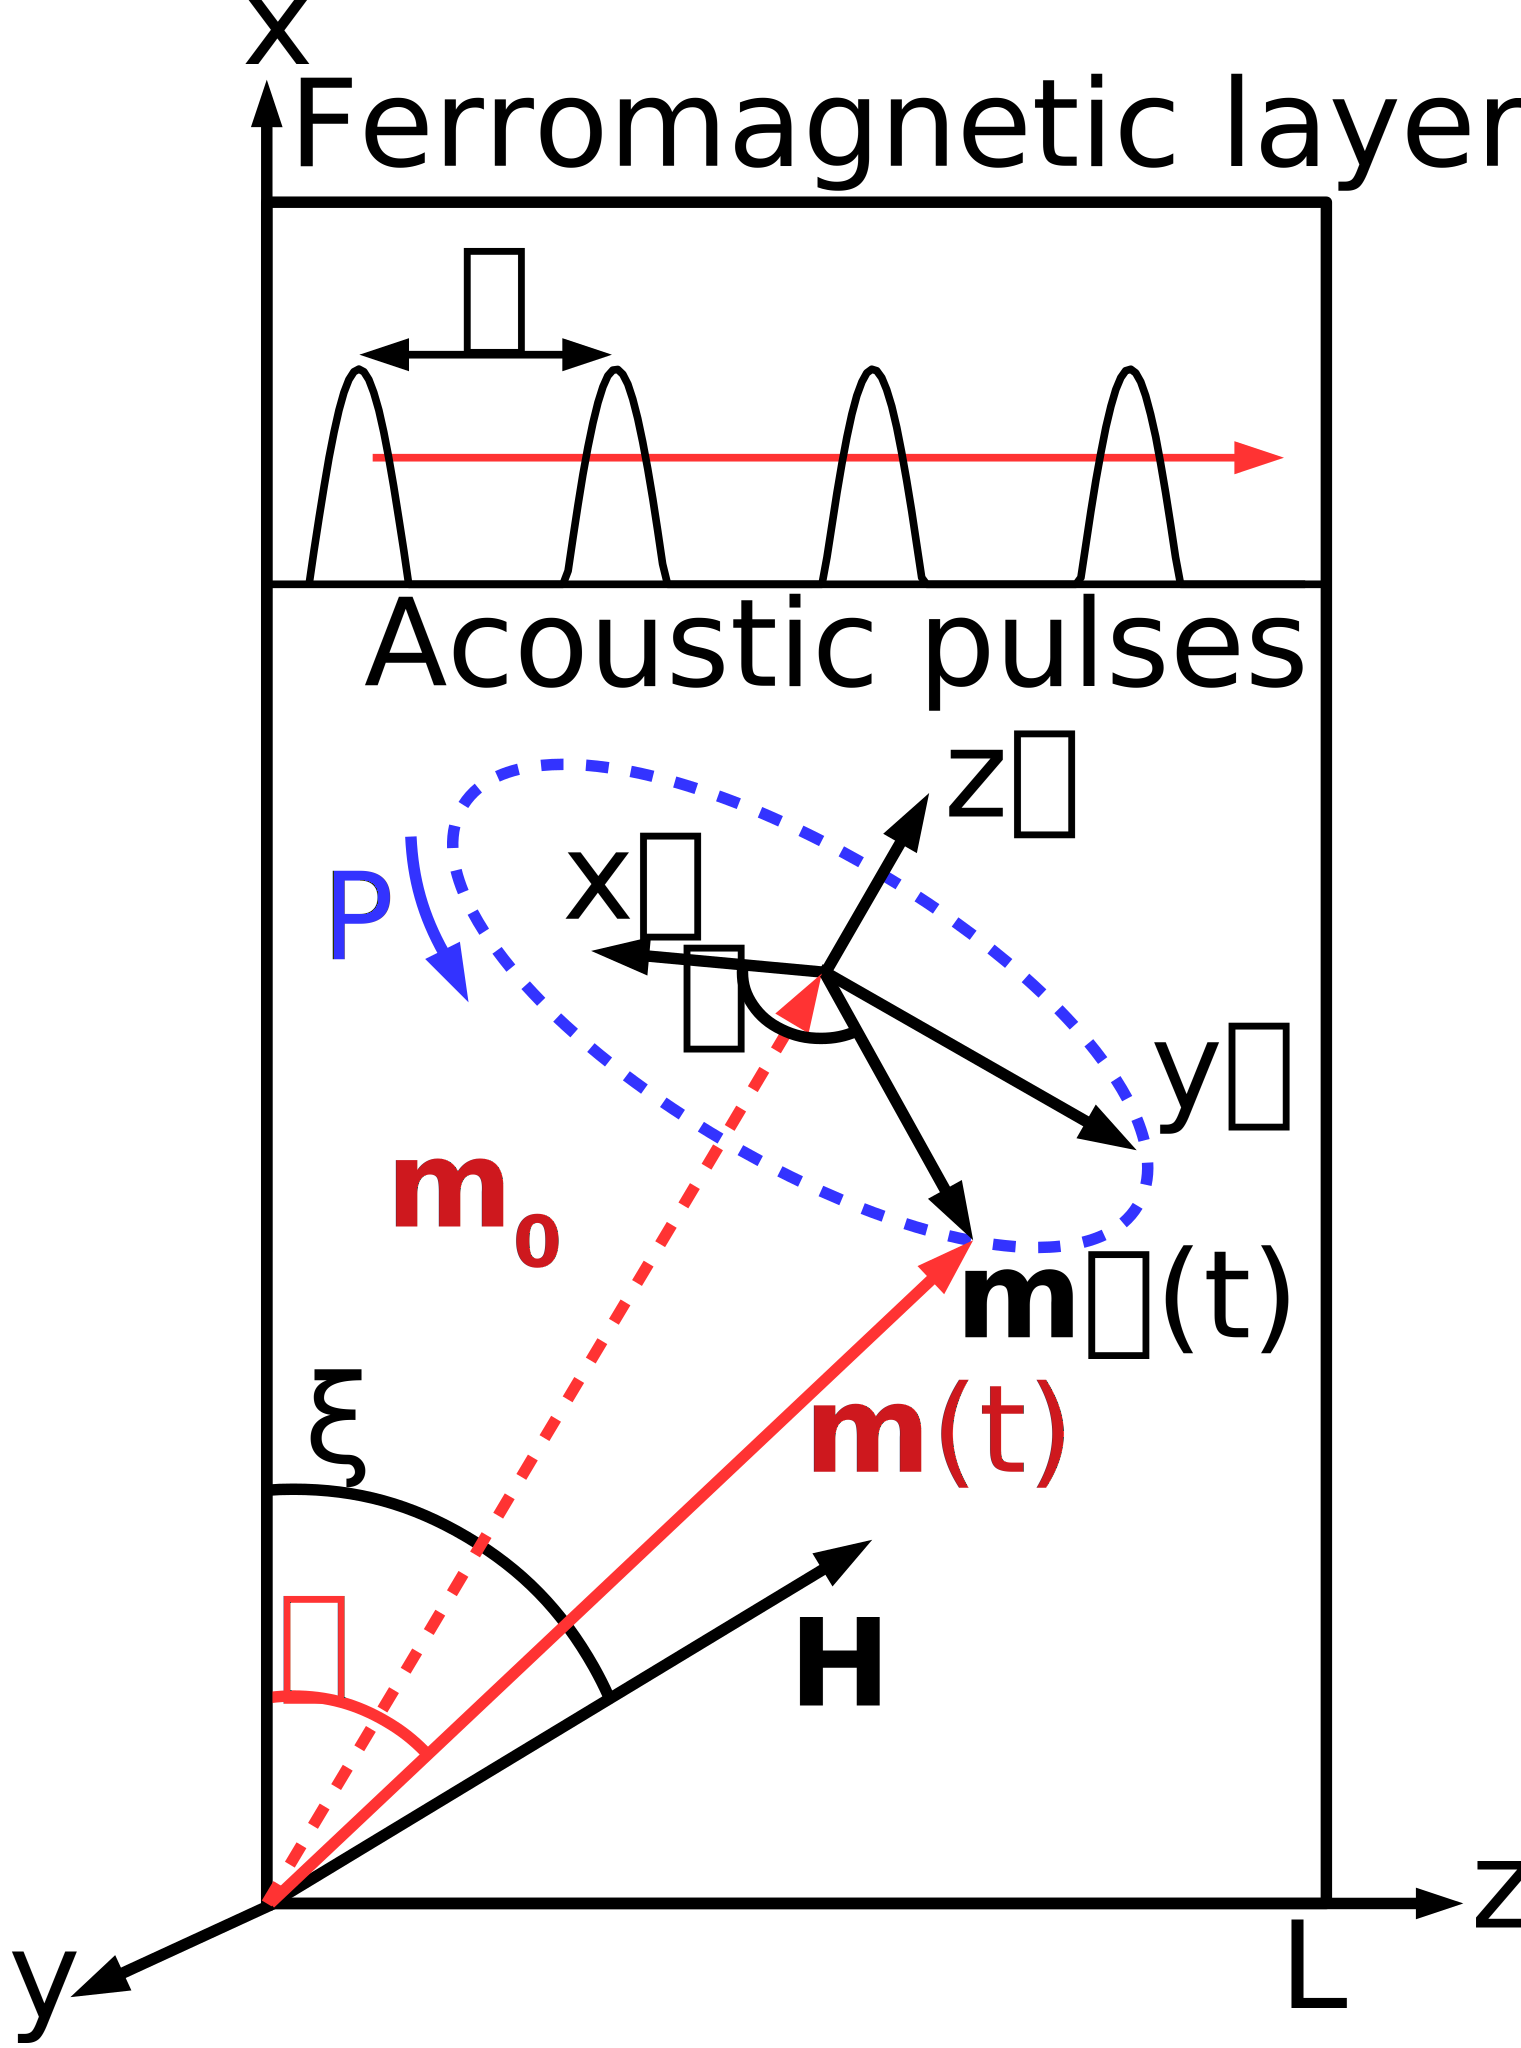
\includegraphics[width=0.4\columnwidth]{geometry_scheme.eps}}
	\hspace{0.1\columnwidth} 
    \subfloat[]{\label{fig:schemeMovement}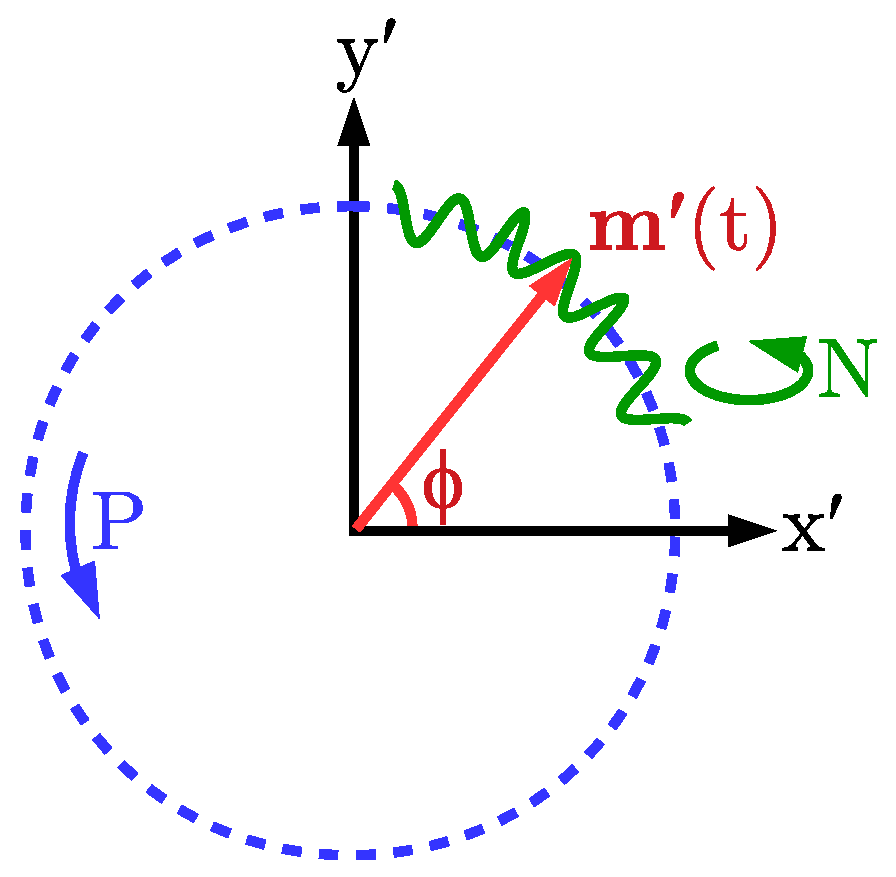
\includegraphics[width=0.4\columnwidth]{Movement.eps}}
	\caption{(Colors online) (a): Geometry of the situation.}
	\label{fig:schemes}
\end{figure}
Fig.~\ref{fig:schemes} shows the geometry of the problem. The thin ferromagnetic film is placed in a DC magnetic field tilted by an angle $\xi$ with respect to the plane of the film. The magnetization vector is represented as a Fourier series in the corresponding modes 
\begin{equation}
	\mathbf{m} = \mathbf{m}_0 + \sum_{n=0}^{N}{\mathbf{m_n}(t)} \cdot \cos{\frac{\pi n}{L}z}
	\label{eq:Fourier}
	%\frac{\alpha}{\left| \mathbf{m}
\end{equation}
where \textit{n} is the magnon mode number, \textit{L} is the thickness of ferromagnetic film. The constant component of the magnetization vector tilted by the theta angle with respect to the \textit{x} axis.  The second-type (free) boundary conditions for the magnetization are given
\begin{equation}
	\left.\frac{\partial \mathbf{m}}{\partial z}\right|_{z=0,L} = 0.
	\label{eq:Boundary_cond}
\end{equation}
Acoustic pulses propagate through a ferromagnetic film and alter the direction of the effective magnetic field thereby driving precessional motion of the magnetization. The effect on the induced magnetization dynamics induced is measured by monitoring the Kerr rotation angle at opposite side of ferromagnetic film.
	
The behavior of the magnetization vector can be estimated through the characteristics of the dispersion curves of acoustic and spinwaves branches. By playing with the magnetic field we can tune the spinwave dispersion curve. So we can choose the magnitude of the field in such a way that there is none, only one or two intersection points between acoustic and spinwave dispersion curves. For the case of one intersection point phase velocity of magnons and acoustic pulses will be equal. In this case the most suitable frequency is close to 500 GHz. It corresponds to a delay of 2 ps between the acoustic pulses.
	
\begin{figure}[ht]
	\centering
	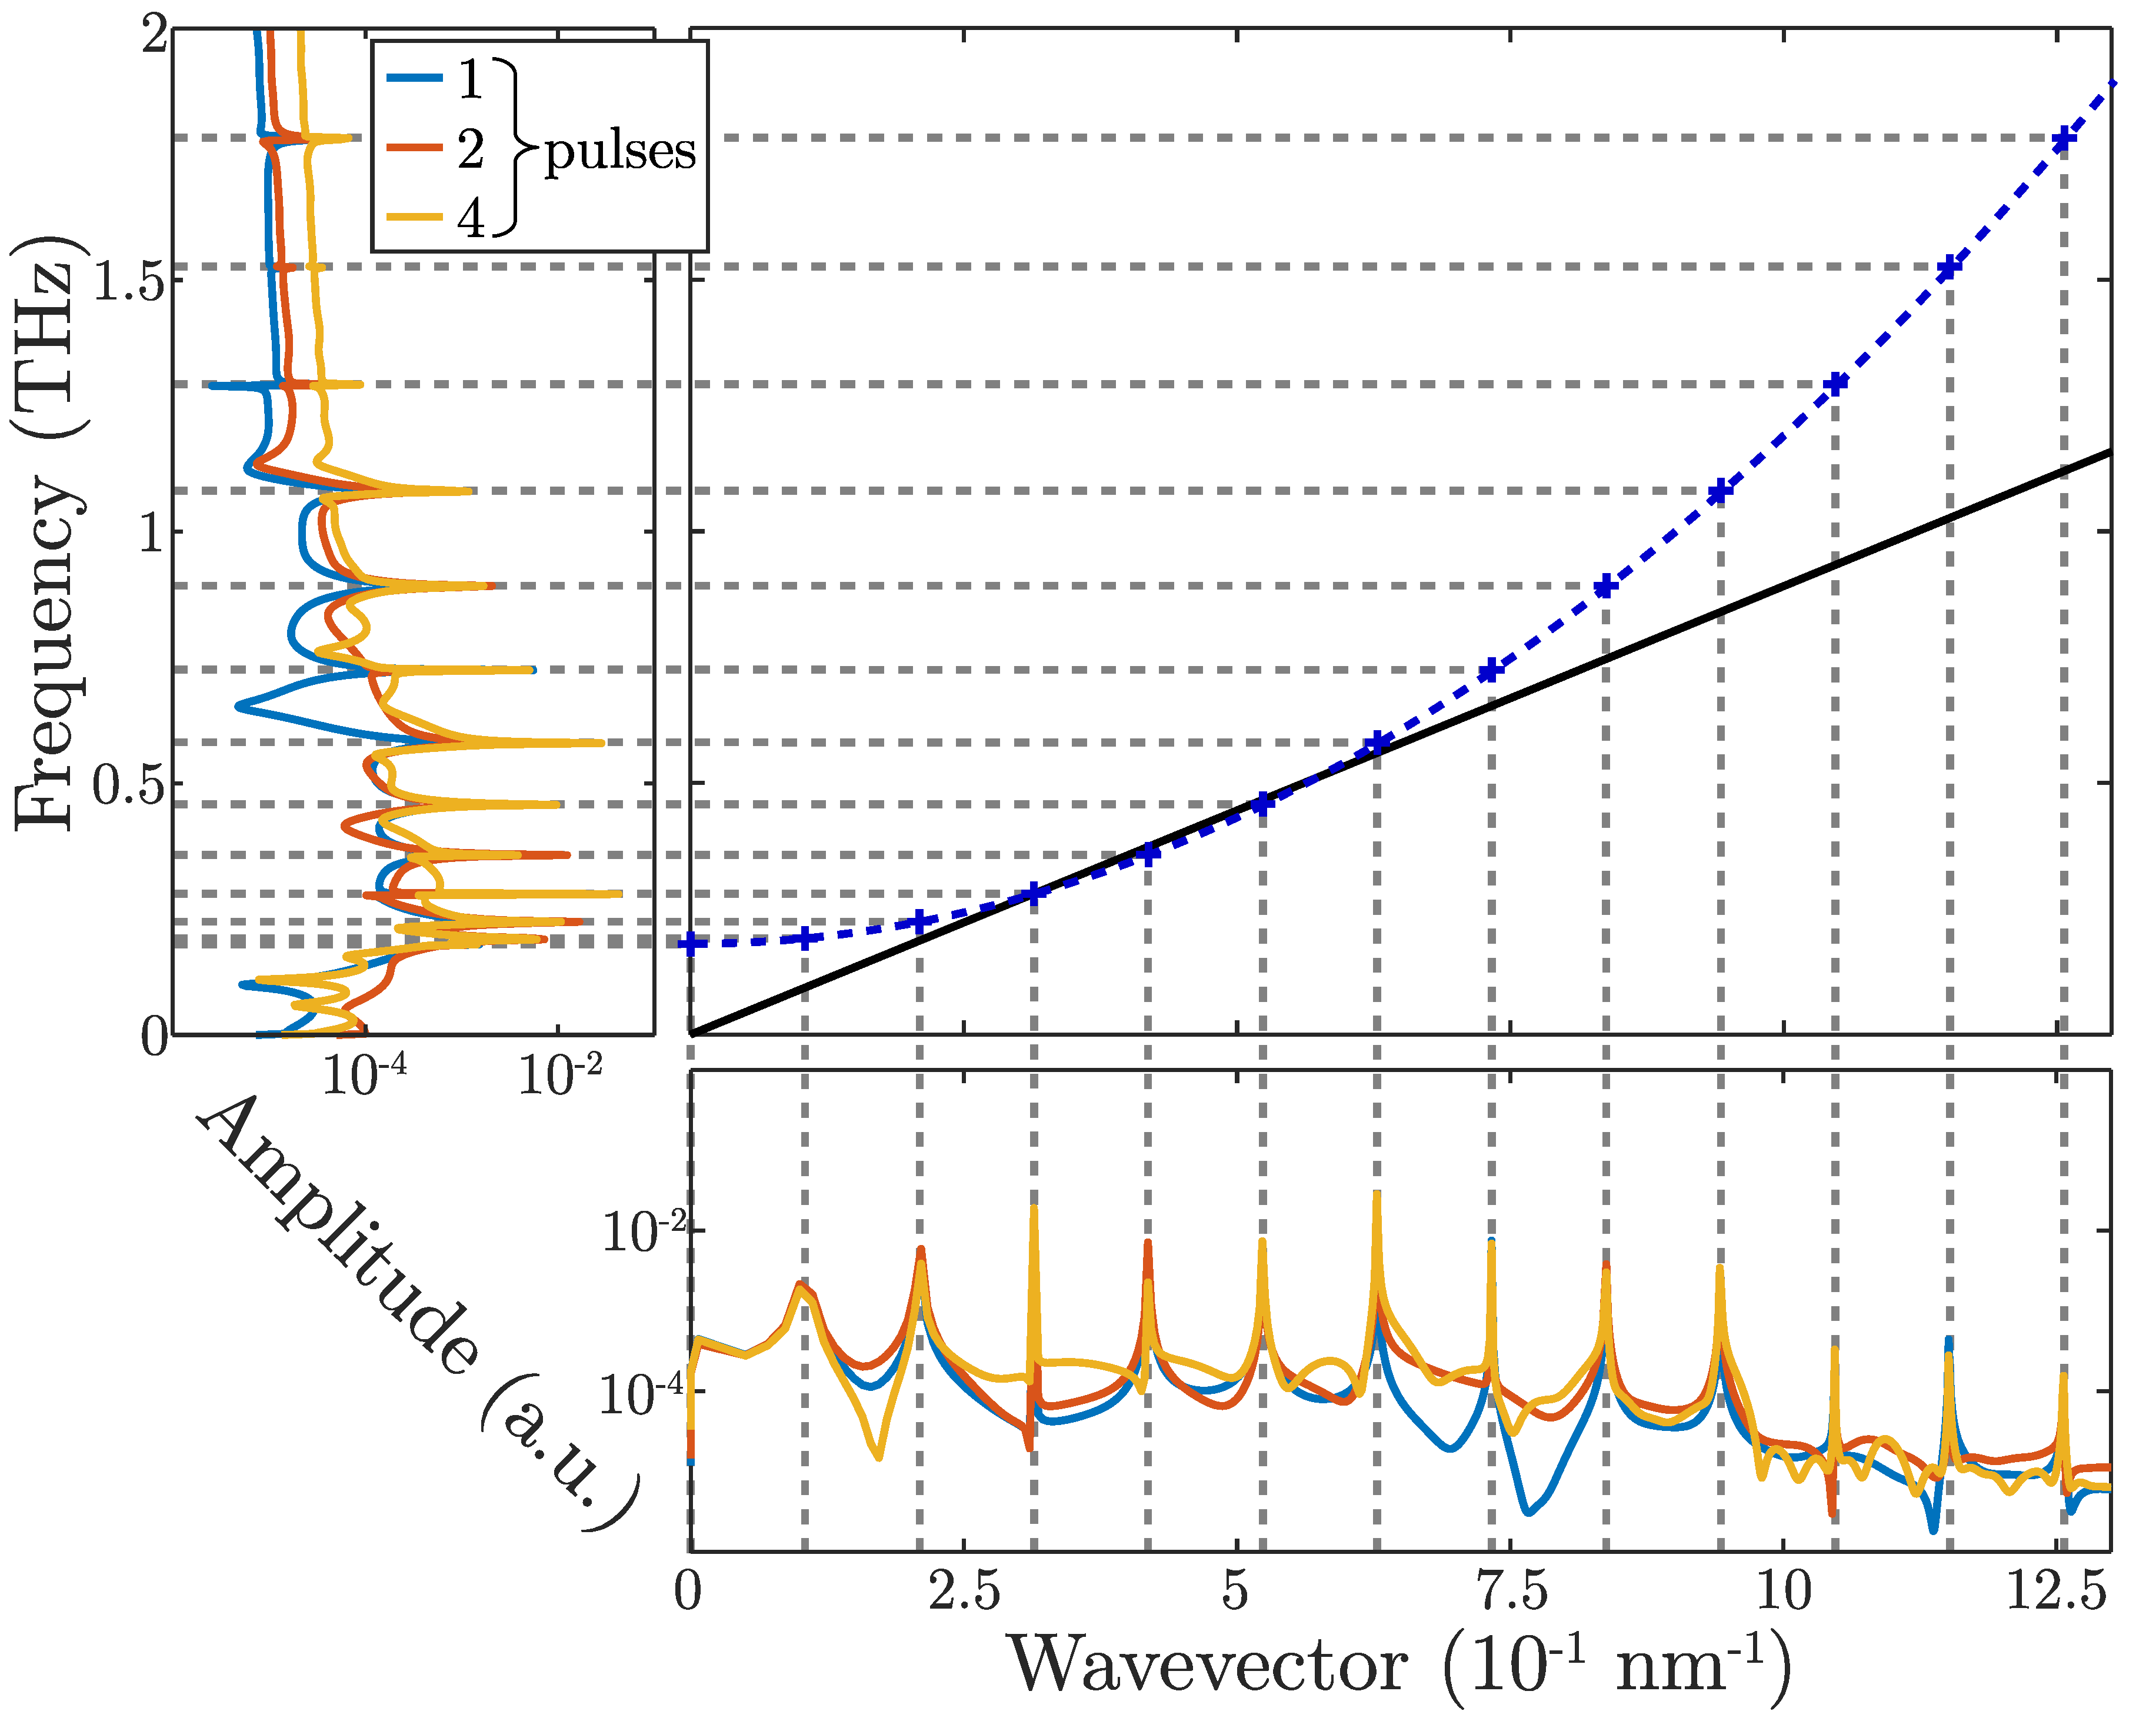
\includegraphics[width=0.95\columnwidth]{Figures/dispersionRelation-H6.5T-Ni30nm-3.57_2ps.eps}
	\caption{Acoustic dispersion relation curve (black line) and magnon dispersion relation curve for $H = 6.5\ \mathrm{T}$ (blue dashed line). The left figure corresponds to the spectrum of the acoustic excitation. The frequencies of acoustic pulses is 280.1 GHz.}
	\label{fig:dispersionRelationHNi}
\end{figure}
	
Acoustic and magnon dispersion relation curves for a magnitude of the DC magnetic field equals to 6.5 T and angle $\xi = 45^{\circ}$  are shown in Fig.~\ref{fig:dispersionRelationHNi}. Two intersection points on the dispersion curves in Fig. 2 can be seen. Parameters of the acoustic pulses that correspond to the left intersection point were taken. The duration of a single acoustic pulse is 1 ps and time between acoustic pulses equals to 3.57 ps which corresponds to the frequency between pulses equals to 280.1 GHz for the case of several pulses in the series.
	
The spectrum of the magnetization dynamics in nickel thin film excited by a series of picosecond acoustic pulses with the parameters described above shown in the left part of Fig.~\ref{fig:dispersionRelationHNi}. The largest contribution to the spectrum was made by the frequency corresponding to the frequency of the intersection point of the acoustic and spinwave dispersion branches regardless of the number of pulses. Subharmonics and harmonics of a higher order are also excited. The frequency difference between adjacent peaks increases linearly with increasing mode number (Fig.~\ref{fig:dF_regularity}).
	
\begin{figure}[ht]
	\centering
	\includegraphics[width=0.95\columnwidth]{dF_regularity.eps}
	\caption{The dependence of frequency difference between adjacent peaks from peak number.}
	\label{fig:dF_regularity}
\end{figure}
	
The amplitude of the excited oscillations can be amplified by increasing the number of acoustic pulses. Changing the number of acoustic pulses and time between them we can strengthen certain harmonics and jam the others. This is significantly determined by the spectrum of the initial acoustic signal and the frequencies present in it.
	
Fig.~\ref{fig:spectrumUniBip} shows the oscillation spectra for series of four acoustic pulses of unipolar and bipolar forms. Excitation occurs at the same frequencies as can be seen from the spectra of the excited oscilations. A unipolar pulses gives a greater contribution to the relatively lower frequencies and bipolar pulses to higher ones. It is determined by the spectrum of the initial acoustic signal. For a unipolar pulses the peak of the spectral dependence is shifted to low frequencies and for the bipolar pulses to high frequencies. This is due to the fact that for the acoustic bipolar pulses of 1 ps duration the maximum in spectrum is close to 1 THz. But since the spectra are similar it is possible to change the amplitude of acoustic pulses to achieve the same effects for certain modes or frequencies as if a transition from a unipolar form of acoustic pulses to a bipolar one were used.
	
\begin{figure}[ht]
	\centering
	\includegraphics[width=0.95\columnwidth]{spectrumLogNorm-Ni_30nm-6_5T-uni_bip-3_57ps-withMode.eps}
	\caption{(Colors online) Unipolar and bipolar.}
	\label{fig:spectrumUniBip}
\end{figure}
	
\begin{figure}[ht]
	\centering
	\includegraphics[width=0.95\columnwidth]{spectrumDampingNormLog-Ni_30nm-6_5T-uni-3_57ps-withMode.eps}
	\caption{(Colors online) Damping.}
	\label{fig:spectrumUniDamping}
\end{figure}
	
The oscillation spectra for series of four unipolar acoustic pulses for different damping parameters $\alpha$ shown on Fig.~\ref{fig:spectrumUniDamping}. The presence of damping significantly affects the shape of the spectral dependence. The highfrequency parts of the excited oscillations decay most rapidly. The oscillation spectrum begins to repeat the spectrum of the initial acoustic signal at large damping parameters.
	
%We studied the excitation of exchange magnons in nickel thin film. By varying the magnitude of the magnetic field It is possible to drive the magnetization with acoustic pulses by playing on their shapes, their number and the delay between them.The spinwaves could be highly damped, making them more difficult to detect.

In conclusion, we reported a study of exchange magnons in nickel thin films excited by a series of picosecond acoustic pulses.
Our model described the generation and the propagation of a spinwave packet due to the propagation of acoustic pulses through the nickel film.
The magnetization dynamics movement can be decomposed in a precession and a nutation movement in the precession's plane.
We demonstrate the we excited high order magnons and it is possible to enhance this excitation by playing on the delay between the successive acoustic pulses in order to match the phase velocity condition.
	
\bigskip
	
Funding through Nouvelle \'{e}quipe, nouvelle th\'{e}matique "Ultrafast acoustics in hybrid magnetic nanostructures", Strat\'{e}gie internationale NNN-Telecom and the Acoustic HUB de la R\'{e}gion Pays de La Loire, Alexander von Humboldt Stiftung, the European Research Council (FP7/2007-2013) / ERC grant agreement no. 306277 and PRC CNRS-RFBR "Acousto-magneto-plasmonics" (grant number 1757 150001) is greatfully acknowledged.
	
\bibliographystyle{apsrev4-1} % Tell bibtex which bibliography style to use
\bibliography{bib_ExchangeMagnons}
	
\end{document}